\documentclass{article}
\usepackage[letterpaper, margin=1in]{geometry}
\usepackage{fixltx2e}
\usepackage{listings}
\usepackage{graphicx} % Required for inserting images
\usepackage{setspace}
\usepackage{multirow}
\usepackage{float}
\usepackage[sorting=none]{biblatex}
\addbibresource{labreport.bib}

\setstretch{1.50}
\title{
\textbf{Laboratory Report} \\
\large Runtime-efficient threaded interpolating elevation of a \emph{n $\times$ n} matrix \emph{M} given a lower resolution digital elevation matrix \emph{N}
}
\author{Jasrel Roby Peralta}
\date{March 2023}

\sloppy
\begin{document}

\maketitle

\section*{Introduction}
\hspace{\parindent} After creating a threaded computer program from Exercise 01, use the programming exercise from Exercise 02 Part 01 to record average runtimes of estimation of a \emph{n $\times$ n} matrix when using a different \emph{t} number of processors.

\section*{Objectives}
The goal for this exercise is the following:
\begin{itemize}
    \item determine the complexity of estimating the point elevation of a \emph{n $\times$ n} square matrix with randomized values at grid points divisible by 10 when using \emph{n} concurrent processors and other values of concurrent processors.
    \item know why the runtime of \emph{t=1} is lower than the average runtime that was obtained in Exercise 01.
    \item figure out why higher values of \emph{n} size of matrix are now possible using \emph{t} concurrent threads.
\end{itemize}

\section*{Methodology} 
\hspace{\parindent} The machine used for this exercise is running on Ubuntu 22.04.2 LTS x86\_64, Intel i-7 8700 (12 cores) @ 4.60GHz, AMD ATI Radeon HD 8570 / RS 430, with 16GB memory. The programming language used in the computer program is Python 3.10.6. The interpolating algorithm used was the Federal Communications Commission (FCC) method. The graphing software used for making the charts is LibreOffice Calc. \\
\indent The computer program made use of the \emph{threading} module of Python 3.10.6, to utilize \emph{t} threads and concurrently estimate different \emph{(n/t) $\times$ n} submatrices from the \emph{n $\times$ n} matrix. \\ 
\indent The size of the matrix for all recorded runs was n = 8000. Moreover, three (3) runs were done using \emph{t} number of processors, starting from 1 (2\textsuperscript{0}) up to 64 (2\textsuperscript{6}). These runs were then averaged and recorded to a table.

\section*{Results and Discussion}
\hspace{\parindent} After running the program three (3) times for each \emph{n} matrix size and \emph{t} concurrent processor combinations, the following table is created:
\begin{table}[H]
    \centering
    \noindent\makebox[\textwidth]{
    \begin{tabular}{|c|c|ccc|c|}
    \hline
    \multirow{2}{*}{\textbf{\begin{tabular}[c]{@{}c@{}}n\\ (size of matrix)\end{tabular}}} & \multirow{2}{*}{\textbf{\begin{tabular}[c]{@{}c@{}}t\\ (number of concurrent threads)\end{tabular}}} & \multicolumn{3}{c|}{\textbf{\begin{tabular}[c]{@{}c@{}}Time Elapsed\\ (seconds)\end{tabular}}} & \multirow{2}{*}{\textbf{\begin{tabular}[c]{@{}c@{}}Average Runtime\\ (secs)\end{tabular}}} \\ \cline{3-5}
                                                                                           &                                                                                                      & \multicolumn{1}{c|}{\textbf{Run 1}}   & \multicolumn{1}{c|}{\textbf{Run 2}}  & \textbf{Run 3}  &                                                                                            \\ \hline
    8000                                                                                   & 1                                                                                                    & \multicolumn{1}{c|}{100.912083}       & \multicolumn{1}{c|}{99.045359}       & 98.716483       & 99.557975                                                                                  \\ \hline
    8000                                                                                   & 2                                                                                                    & \multicolumn{1}{c|}{106.021552}       & \multicolumn{1}{c|}{107.055136}      & 105.227246      & 106.101311333333                                                                           \\ \hline
    8000                                                                                   & 4                                                                                                    & \multicolumn{1}{c|}{108.299674}       & \multicolumn{1}{c|}{107.104734}      & 107.16318       & 107.522529333333                                                                           \\ \hline
    8000                                                                                   & 8                                                                                                    & \multicolumn{1}{c|}{114.795173}       & \multicolumn{1}{c|}{113.608294}      & 122.527366      & 116.976944333333                                                                           \\ \hline
    8000                                                                                   & 16                                                                                                   & \multicolumn{1}{c|}{119.669082}       & \multicolumn{1}{c|}{118.507086}      & 119.356774      & 119.177647333333                                                                           \\ \hline
    8000                                                                                   & 32                                                                                                   & \multicolumn{1}{c|}{124.609196}       & \multicolumn{1}{c|}{124.346253}      & 122.94652       & 123.967323                                                                                 \\ \hline
    8000                                                                                   & 64                                                                                                   & \multicolumn{1}{c|}{125.016126}       & \multicolumn{1}{c|}{130.814412}      & 125.503346      & 127.111294666667                                                                           \\ \hline
    \end{tabular}}
    \caption{\label{table}Average runtimes of the computer program from 1 to 64 concurrent threads}
    \end{table}

\indent To further visualize the values obtained from the execution of the computer program, a line graph was created. 
\begin{figure}[H]
    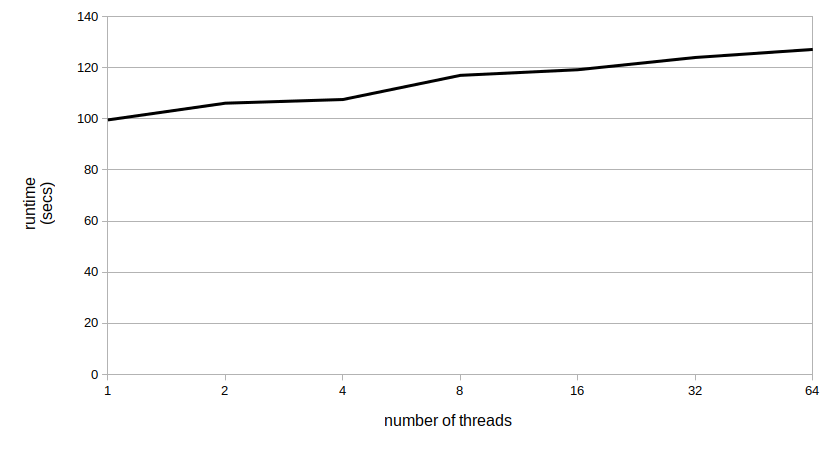
\includegraphics[width=0.8\textwidth]{chart01.png}
    \centering
    \caption{Line Chart of the Average runtimes of the computer program from 1 to 64 concurrent threads}
    \end{figure}

\indent As seen in Figure 1, the running time of the code gets higher as it gets a higher amount of threads working on the estimation of the elevation points of the \emph{n $\times$ n} matrix. The possible reason for this could be the Global Interpreter Lock (GIL) feature on Python 3 \cite{intro, gil}. With GIL, only one thread of Python code at a time can be run. Though it limits the multithreading capabilities of the programming language, it said that it improves the execution times for single-threaded programs \cite{thread-based}. A possible solution for this would be to use the \emph{multiprocessing} Python module \cite{multiprocessing} which utilizes subprocesses rather than threads.
\begin{table}[H]
    \noindent\makebox[\textwidth]{
        \begin{tabular}{|c|c|ccc|c|}
        \hline
        \multirow{2}{*}{\textbf{\begin{tabular}[c]{@{}c@{}}n\\ (size of matrix)\end{tabular}}} & \multirow{2}{*}{\textbf{\begin{tabular}[c]{@{}c@{}}t\\ (number of concurrent threads)\end{tabular}}} & \multicolumn{3}{c|}{\textbf{\begin{tabular}[c]{@{}c@{}}Time Elapsed\\ (seconds)\end{tabular}}} & \multirow{2}{*}{\textbf{\begin{tabular}[c]{@{}c@{}}Average Runtime\\ (secs)\end{tabular}}} \\ \cline{3-5}
                                                                                            &                                                                                                         & \multicolumn{1}{c|}{\textbf{Run 1}}   & \multicolumn{1}{c|}{\textbf{Run 2}}  & \textbf{Run 3}  &                                                                                            \\ \hline
        8000                                                                                   & 125                                                                                                     & \multicolumn{1}{c|}{128.8022}         & \multicolumn{1}{c|}{127.379904}      & 119.941635      & 125.374579666667                                                                           \\ \hline
        8000                                                                                   & 250                                                                                                     & \multicolumn{1}{c|}{124.561448}       & \multicolumn{1}{c|}{128.594597}      & 125.536152      & 126.230732333333                                                                           \\ \hline
        8000                                                                                   & 500                                                                                                     & \multicolumn{1}{c|}{117.321256}       & \multicolumn{1}{c|}{119.474981}      & 118.826453      & 118.540896666667                                                                           \\ \hline
        8000                                                                                   & 1000                                                                                                    & \multicolumn{1}{c|}{111.385769}       & \multicolumn{1}{c|}{111.77902}       & 116.368289      & 113.177692666667                                                                           \\ \hline
        8000                                                                                   & 2000                                                                                                    & \multicolumn{1}{c|}{94.508929}        & \multicolumn{1}{c|}{95.83168}        & 99.262235       & 96.5342813333333                                                                           \\ \hline
        8000                                                                                   & 4000                                                                                                    & \multicolumn{1}{c|}{66.444255}        & \multicolumn{1}{c|}{68.056844}       & 71.336607       & 68.6125686666667                                                                           \\ \hline
        8000                                                                                   & 8000                                                                                                    & \multicolumn{1}{c|}{10.386343}        & \multicolumn{1}{c|}{10.333371}       & 9.87454         & 10.1980846666667                                                                           \\ \hline
        \end{tabular}
    }
    \caption{\label{table}Average runtimes of the computer program from 125 to \emph{n} concurrent threads}
    \end{table}

\indent However, the average runtime decreases after running the code with higher \emph{t} number of concurrent threads. The highest average runtime was observed at 64. A possible reason for this trend could be the execution time that it takes to access the matrix (memory) multiple times. Higher amount of threads makes it handle less amount of data since a thread will be assigned to lower values of columns. On the other hand, this could also be the reason why the runtime is also low when using a small \emph{t} number of threads, since all data needed for estimation of point elevations are already available and multiple matrix (memory) accesses are not needed. A line graph is created to further visualize the trend previously mentioned.
\begin{figure}[H]
    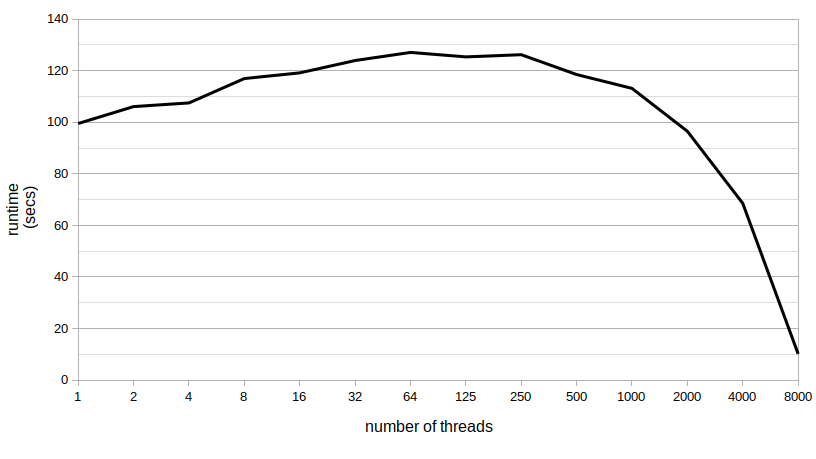
\includegraphics[width=0.8\textwidth]{chart02.png}
    \centering
    \caption{Line Chart of the Average runtimes of the computer program from 125 to \emph{n} concurrent threads}
    \end{figure}
    
\indent As seen in Figure 2, the average runtime of the computer program started low, and it grew as the number of threads increased. The running time of the threaded computer program at \emph{t = 1} is also faster than the average runtime obtained from Exercise 01. The reason for this could be because all computations are then handled by a single thread and execute all the estimation of all columns by itself. And the execution of the program is the only process the thread has to finish. Compared to running the program serially during Exercise 01, wherein the process has to maximize the memory allocated along with other processes. \\
\indent Furthermore, it is evident in Figure 2 that the average runtime started to decrease when using a higher number of threads, and the runtime when using \emph{n} concurrent threads to estimate point elevations of a \emph{n $\times$ n} matrix drastically decreased. The running time of the algorithm that uses \emph{n} threads in estimating the point elevation of a \emph{n $\times$ n} matrix will be O(n) since each column item will be needed to iterate through only once, because each processor will be assigned to a single column. With this, it can be said that using n/2 concurrent processors will result in a theoretical runtime of O((n\textsuperscript{2})/2), because each processor will be assigned to two (2) columns to estimate concurrently with other processors. And when using n/4 concurrent processors, the theoretical runtime will then be O((n\textsuperscript{2})/4). With these, it can be said that the theoretical runtime using i concurrent processors will be O((n\textsuperscript{2})/i), which is still considered to be O(n\textsuperscript{2}).


\section*{Conclusion}
\hspace{\parindent} The complexity of estimating the point elevation of a \emph{n $\times$ n} square matrix with randomized values at grid points divisible by 10 when using n concurrent processors and other values of concurrent processors is O(n) because each column is iterated through only once, since each column will be assigned to a single processor (thread). \\
\indent The running time of the threaded computer program at \emph{t = 1} is faster than the average runtime obtained from Exercise 01. The reason for this could be because all computations are then handled by a single thread and execute all the estimation of all columns by itself. And the execution of the program is the only process the thread has to finish. Compared to running the program serially during Exercise 01, wherein the process has to maximize the memory allocated along with other processes.\\ 
\indent Dealing with larger matrix sizes is also possible through the use of multiple concurrent threads, as seen in Figure 1, and Figure 2. By assigning a processor for a small number of columns, the runtime of the computer program is lower. However, when using neither a high amount of concurrent threads nor a low amount of concurrent threads, the runtime of the program tends to be high, since more matrix (memory) access is being done. By assigning the right amount of threads to use for estimating point elevations, the average runtime is expected to be lower.\\


\printbibliography{}


\pagebreak
\section*{\centering Appendix}
\begin{center}
Interpolation Source Code \\ (main.py)
\end{center}
\setstretch{1}
\begin{lstlisting}[language=Python]
    import numpy as np
    import random
    import datetime
    import threading
    
    # prettier printing options
    np.set_printoptions(formatter={'float': '{: 0.3f}'.format})
    
    # for given example in exer file
    # mat[0][0] = 200
    # mat[0][10] = 250
    # mat[10][0] = 280
    # mat[10][10] = 300
    
    # interpolate function
    def terrain_inter(mat):
        for i in range(0,n):
            for j in range(0,n):
                if mat[i][j] != 0:
                    continue
                if (i % dist == 0):
                    get_row_val(i,j)
        for i in range(0,n):
            for j in range(0,n):
                if (mat[i][j] == 0):
                    get_col_val(i,j)
        print("\n")
    
    # modified interpolation function
    # to run concurrently with other threads
    # from other x1 to x2's
    def terrain_inter_threaded(mat,x1,x2):
        for i in range(0,n):
            for j in range(x1,x2):
                if mat[i][j] != 0:
                    continue
                if (i % dist == 0):
                    get_row_val(i,j)
        for i in range(0,n):
            for j in range(x1,x2):
                if (mat[i][j] == 0):
                    get_col_val(i,j)
    
    def get_submatrices(n,t):
        # array of submatrices
        sub_arr = []
        temp = []
        for i in range(0,n):
            temp.append(i)
            if (len(temp) == (n-1) / t):
                sub_arr.append(temp)
                temp = []
    
        return sub_arr
    
    # get size of matrix
    def getSize():
        n = 1
        while (n % 10 != 0):
            n = int(input("enter size of matrix: "))
            if n % 10 != 0:
                print('invalid size of matrix')
        return n+1
    
    # get number of threads
    def getThreads(n):
        n -= 1
        t = 0
        # n size should be less than t threads
        # t threads should not be 0
        # n size should be divisible by t threads
        while (n < t) or (t == 0) or (n % t != 0):
            t = int(input('enter number of threads: '))
            if (n < t) or (n % t != 0):
                print('invalid number of threads')
        return t
    
    # dp array format:
    # dp = [[x1,y1][x2,y2]]
    
    # interpolate rows with random values
    def get_row_val(i,j):
        dp = get_datapoints_row(i,j)
        x = j               # j -> row
        x1 = dp[0][0]
        x2 = dp[1][0]
        y1 = dp[0][1]
        y2 = dp[1][1]
        res = fcc(x1,y1,x2,y2,x)
        mat[i][j] = res
    
    # interpolate columns
    def get_col_val(i,j):
        dp = get_datapoints_col(i,j)
        # dp = [[x1,y1][x2,y2]]
        x = i               # i -> col
        x1 = dp[0][0]
        x2 = dp[1][0]
        y1 = dp[0][1]
        y2 = dp[1][1]
        res = fcc(x1,y1,x2,y2,x)
        mat[i][j] = res
    
    
    # get closest datapoints to the current gridpoint
    def get_datapoints_row(i,j):
        dp = []
        dp.append(get_nearest_row(i,j,-1))
        dp.append(get_nearest_row(i,j,+1))
        return dp
    def get_datapoints_col(i,j):
        dp = []
        dp.append(get_nearest_col(i,j,-1))
        dp.append(get_nearest_col(i,j,+1))
        return dp
    
    # x, y -> point; dir -> direction 
    # change direction to check to the nearest 10
    ## improved from recursion from previous exercise to direct computation
    def get_nearest_row(i,j,dir):
        # go up
        if dir < 0:
            dir = j - (j % 10)
        # go down
        else:
            dir = j + (10 - (j % 10))
        return [dir,mat[i][dir]]
    
    def get_nearest_col(i,j,dir):
        # go left
        if dir < 0:
            dir = i - (i % 10)
        # go right
        else:
            dir = i + (10 - (i % 10))
        return [dir,mat[dir][j]]
    
    # follow given FCC formula
    def fcc(x1,y1,x2,y2,x):
        return (y1 + (((x-x1)/(x2-x1)) * (y2-y1)))
    
    # main function
    if __name__ == "__main__":
        # initialize data
        n = getSize()
        t = getThreads(n)
    
        # distance between randomized values
        dist = 10
    
        # # create a zero nxn matrix
        # mat = np.zeros((n,n), dtype = float)
    
        # # randomize elevation values for gridpoints divisible by 10
        # for i in range(n):
        #     for j in range(n):
        #         if i % dist == 0 and j % dist == 0:
        #             mat[i][j] = random.uniform(0.0, 1000.0)
    
        # # print initial matrix
        # print(mat)
    
        # # record time before serial interpolation
        # time_before_serial = datetime.datetime.now()
    
        # # interpolate matrix
        # terrain_inter(mat)
    
        # # record time after serial interpolation
        # time_after_serial = datetime.datetime.now()
    
    
        # # print resulting matrix
        # print(mat)
    
        # print("\n\n\n")
    
    
        # create a zero nxn matrix
        mat = np.zeros((n,n), dtype = float)
    
        # randomize elevation values for gridpoints divisible by 10
        for i in range(n):
            for j in range(n):
                if i % dist == 0 and j % dist == 0:
                    mat[i][j] = random.uniform(0.0, 1000.0)
    
        # print initial matrix
        print(mat)
    
        threads = list()
    
        for set in get_submatrices(n,t):
            x1, x2 = set[0], set[-1]
            thread = threading.Thread(target=terrain_inter_threaded, args=(mat,x1,x2))
            threads.append(thread)
    
        # record time before threaded interpolation
        time_before_parallel = datetime.datetime.now()
    
    
        for thread in threads:
            thread.start()
    
        for thread in threads:
            thread.join()
    
        # record time after threaded interpolation
        time_after_parallel = datetime.datetime.now()
    
    
        # print resulting matrix
        print(mat)
    
        # print interpolation time
        # print("serial: ",time_after_serial-time_before_serial)
        print("parallel: ",time_after_parallel-time_before_parallel)
\end{lstlisting}

\end{document}
